\subsection{Configurazione Collegamento al Server}\label{CCS}

Una volta aggiunto alla dashboard di \textit{Grafana} il pannello \textit{G\&B} (§\ref{AddPanel}), per poter interagire in modo efficace con il pannello è necessaria, come prima operazione, configurare il collegamento al server, che è il componente che si occupa delle operazioni di ricalcolo delle probabilità. Tale operazione funge da precondizione per ogni altra funzionalità del prodotto.\\
Per poter effettuare l'operazione in esame, l'utente deve innanzittuto accedere all'apposita sezione del menù di Edit del pannello, attraverso il percorso \textbf{Edit > Visualization} (Figura \ref{EditMenu}). Si ricorda che il menù di edit può essere acceduto cliccando il nome del pannello e selezionando "Edit", oppure semplicemente attraverso il click del tasto "e".

\begin{figure}[H]
	\begin{center}
		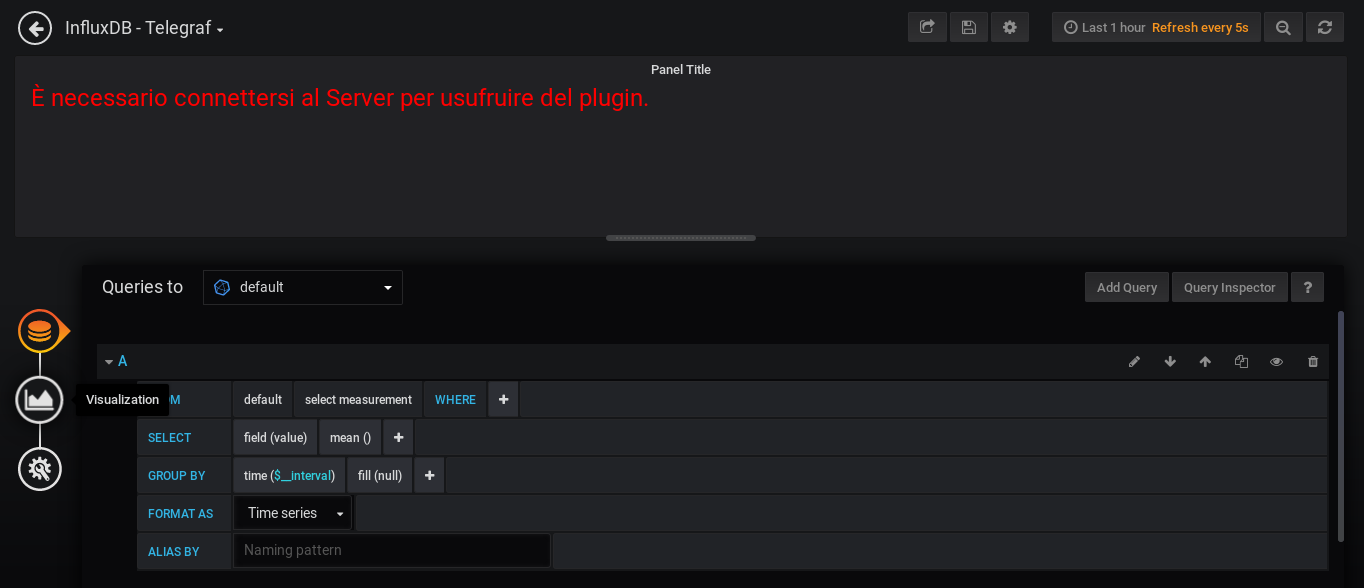
\includegraphics[scale=0.31]{./images/VisualizServerSettings.png}
		 \caption{Menù di Edit del Pannello \textit{G\&B}}	
		 \label{EditMenu}
	\end{center}
\end{figure}

Una volta selezionata la "tab" \textbf{Visualization} all'utente verrà dunque chiesto di inserire, negli appositi campi dati indicati in Figura \ref{ServerSettings}:
\begin{enumerate}
	\item Indirizzo IP del Server;
	\item Porta del Server in ascolto.
\end{enumerate}
Una volta editati i campi dati indicati, l'utente deve confermare le proprie scelte premendo il pulsante \textbf{Connetti}.\\

\begin{figure}[H]
	\begin{center}
		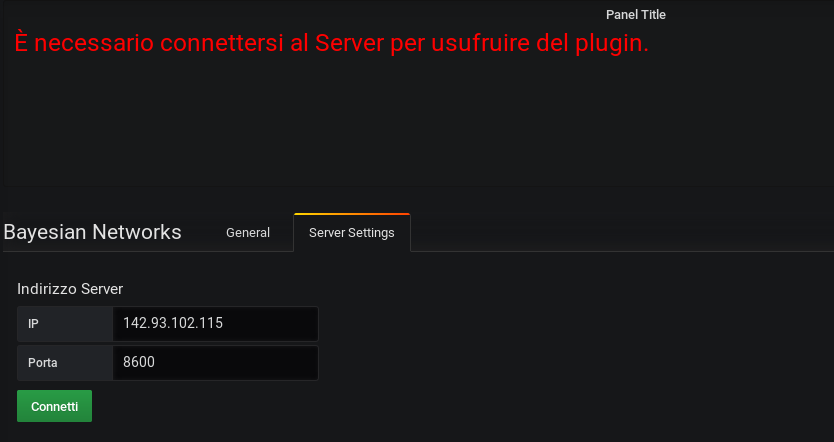
\includegraphics[scale=0.37]{./images/ServerSettings.png}
		 \caption{Sezione "Server Settings" del menù di Edit del Pannello \textit{G\&B}}	
		 \label{ServerSettings}
	\end{center}
\end{figure}

Nel caso in cui il cui la configurazione del server sia andata a buon fine, l'utente viene avvisato dell'avvenuto collegamento attraverso un messaggio di notifica (Figura \ref{NotificaServer}).

\begin{figure}[H]
	\begin{center}
		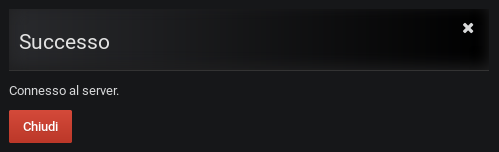
\includegraphics[scale=0.6]{./images/NotificaServer.png}
		 \caption{Notifica di avvenuto collegamento del Server}	
		 \label{NotificaServer}
	\end{center}
\end{figure}

~\\
\textbf{\textcolor{red}{ATTENZIONE}}: Nel caso in cui l'utente abbia commesso degli errori in fase di compilazione dei campi dati, l'operazione non va a buon fine e l'utente viene avvisato degli errori commessi da un messaggio di errore (Figura \ref{ErroreServer}).

\begin{figure}[H]
	\begin{center}
		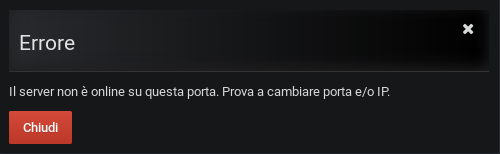
\includegraphics[scale=0.6]{./images/ErroreServer.png}
		 \caption{Messaggio di Errore configurazione Server}	
		 \label{ErroreServer}
	\end{center}
\end{figure}


Una volta configurato correttamente il collegamento al server, l'utente ha accesso alla \textbf{vista principale} del plug-in:
\begin{figure}[H]
	\begin{center}
		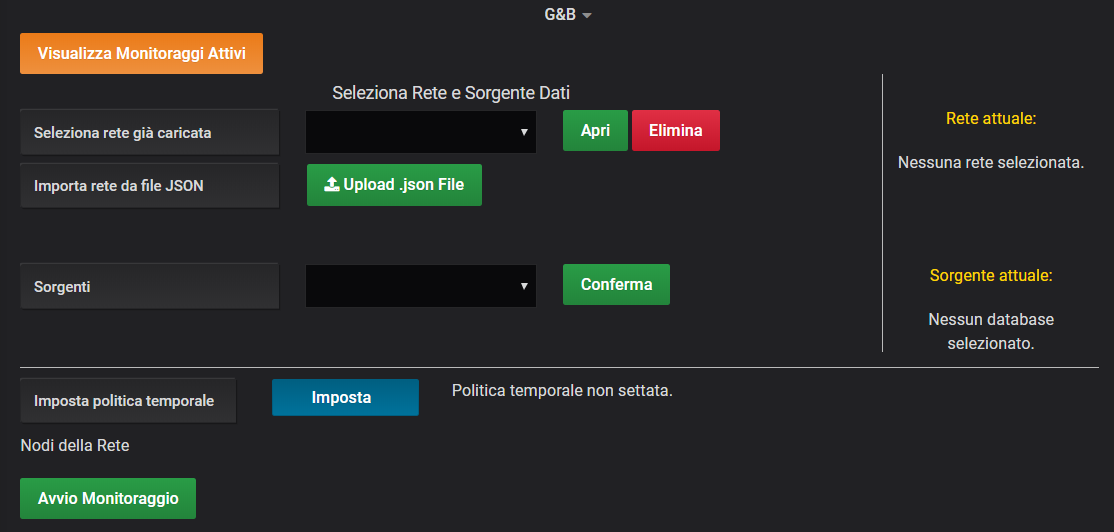
\includegraphics[scale=0.64]{./images/Panel.png}
		 \caption{Vista Principale delle Impostazioni di Collegamento del Pannello \textit{G\&B}}	
		 \label{Pannello}
	\end{center}
\end{figure}

Nello specifico la Figura \ref{Pannello} raffigura la sezione deputata alla definizione delle Impostazioni di Collegamento della rete bayesiana al flusso dati, a cui l'utente ha immediatamente accesso.
